%% LyX 2.1.4 created this file.  For more info, see http://www.lyx.org/.
%% Do not edit unless you really know what you are doing.
\documentclass[10pt,UTF8]{report}
\usepackage[T1]{fontenc}
\usepackage{geometry}
\geometry{verbose,tmargin=3cm,bmargin=3cm,lmargin=2.7cm,rmargin=2.7cm}
\usepackage{fancyhdr}
\pagestyle{fancy}
\setcounter{secnumdepth}{3}
\setcounter{tocdepth}{1}
\usepackage{color}
\usepackage{float}
\usepackage{mathtools}
\usepackage{amsmath}
\usepackage{amssymb}
\usepackage{cancel}
\usepackage{mathdots}
\usepackage{stmaryrd}
\usepackage{stackrel}
\usepackage{graphicx}
\PassOptionsToPackage{version=3}{mhchem}
\usepackage{mhchem}
\usepackage{esint}
\usepackage[unicode=true,
 bookmarks=true,bookmarksnumbered=true,bookmarksopen=true,bookmarksopenlevel=1,
 breaklinks=true,pdfborder={0 0 1},backref=false,colorlinks=true]
 {hyperref}
\hypersetup{pdftitle={A Preliminary Implementation of Linux Kernel Virus and Process Hiding},
 pdfauthor={Junru Shao, Jian Weng, Yan Ji},
 pdfkeywords={Security, Process, VFS, IO, LKM},
 CJKbookmarks, linkcolor = red, anchorcolor = blue, citecolor = green}

\makeatletter

%%%%%%%%%%%%%%%%%%%%%%%%%%%%%% LyX specific LaTeX commands.
%% Because html converters don't know tabularnewline
\providecommand{\tabularnewline}{\\}

%%%%%%%%%%%%%%%%%%%%%%%%%%%%%% User specified LaTeX commands.
\usepackage{ctex}
\usepackage{authblk}
\definecolor{grey}{rgb}{0.1,0.1,0.1}

\usepackage{tikz}
\usetikzlibrary{arrows,automata}

\author{邵俊儒\thanks{学号: 5130309028}~~~~翁健\thanks{学号: 5130309033}~~~~吉妍\thanks{学号: 5130309067}}
\affil{\small{ACM Honored Class\\ Zhiyuan College \\ Shanghai Jiao Tong University} }

\definecolor{mygray}{rgb}{0.5,0.5,0.5}

\RequirePackage[framemethod=default]{mdframed} % Required for creating the theorem, definition, exercise and corollary boxes
\newmdenv[skipabove=7pt,
skipbelow=7pt,
rightline=false,
leftline=true,
topline=false,
bottomline=false,
linecolor=gray,
backgroundcolor=black!5,
innerleftmargin=5pt,
innerrightmargin=5pt,
innertopmargin=-4pt,
innerbottommargin=-12pt,
leftmargin=0cm,
rightmargin=0cm,
linewidth=4pt]{codeBox}
\newenvironment{code}[1]{\begin{codeBox}\begin{lstlisting}[language=#1]}{\end{lstlisting}\end{codeBox}}

\makeatother

\usepackage{listings}
\lstset{basicstyle={\ttfamily\small},
frame=none,
keepspaces=true,
columns=spaceflexible,
breaklines=true,
breakindent=0pt,
extendedchars=false,
keywordstyle={\color{blue!70}},
commentstyle={\color{red!50!green!50!blue!50}},
rulesepcolor={\color{red!20!green!20!blue!20}},
escapechar={`}}
\renewcommand{\lstlistingname}{Listing}

\begin{document}

\title{\textbf{A Preliminary Implementation of Linux Kernel Virus and Process
Hiding}}


\author{邵俊儒\thanks{学号: 5130309028}\qquad{}翁健\thanks{学号: 5130309033}\qquad{}吉妍\thanks{学号: 5130309067}}


\date{\today}
\maketitle
\begin{abstract}
\qquad{}结合课堂知识, 我们设计了一个 Linux 内核病毒, 该病毒同时具有木马的自动性, rootkit 的隐蔽性和蠕虫的感染能力.
该病毒获得权限后, 会自动将自身加入 Linux 内核模块中, 劫持 Linux 的系统调用, 并通过简单的方法实现自身的隐蔽. 有两种情况会导致病毒的发作:
第一种, 病毒会自动选择一些进程进行隐藏; 第二种, 用户新建文件夹时, 温和地打印出被截获的命令的进程 ID 和用户的 ID. 该病毒通过移动存储设备进行传播.
具体地, 当移动设备被卸载前, 病毒会及时对该设备进行必要的感染. 本文重视理论与实践的结合, 每一部分都会按照先理论后实践的顺序展开:
首先介绍病毒各个模块的思想, 随后对略有难度的实践细节加以提示. 此外, 本文的全部内容均在 64 位 x86\_64 架构的 Linux
2.6.32-21 内核下测试通过\footnote{选择 64 位架构是为了增加项目难度, 显示原创性, 并展示该病毒蕴含思想的普适性.}.
值得一提的是, 本文病毒所蕴含的思想方法极其简洁, 这使得类似的做法甚至能够在 Linux 3.{*} 版本的内核上顺利运行.

\vspace{2cm}

\noindent  \textbf{关键词}: 安全~进程~文件系统~输入输出~内核~LKM
\end{abstract}
\tableofcontents{}

\newpage{}


\chapter{概述}



\vspace*{2cm}

\textit{We come from an environment molded from 3 billion years of
evolution, and when we change our behavior, there may be problems.}

\begin{flushright}
—— W. Richard Stevens
\par\end{flushright}

\newpage{}

Linux 是一款自由的多用户、多任务的操作系统内核. Linux 能够稳定高效地运行在包括 PC、工作站、服务器等各种平台上. 它对
UNIX 和 POSIX 标准的兼容, 对 GPL 协议和开源精神的恪守, 为它带来了源源不断的生机. 经过多年的发展壮大, 如今
Linux 已经成为服务器端的主流操作系统.

为了提高硬件兼容性, 搭载的各种定制的硬件, 并提供个性化的功能, Linux 引入了可动态装载的内核模块, 即 loadable
kernel module (LKM). 然而, LKM 程序运行在内核态中, 为不少病毒提供了可乘之机.

我们小组编写了一个短小的 LKM 病毒. 该病毒完整地实现了隐藏、传播、感染和破坏四大步骤. 图 \ref{fig:=0075C5=006BD2=005DE5=004F5C=00539F=007406=006D41=007A0B=00793A=00610F=0056FE}
是该病毒传播的简略流程.

\begin{figure}
\begin{centering}
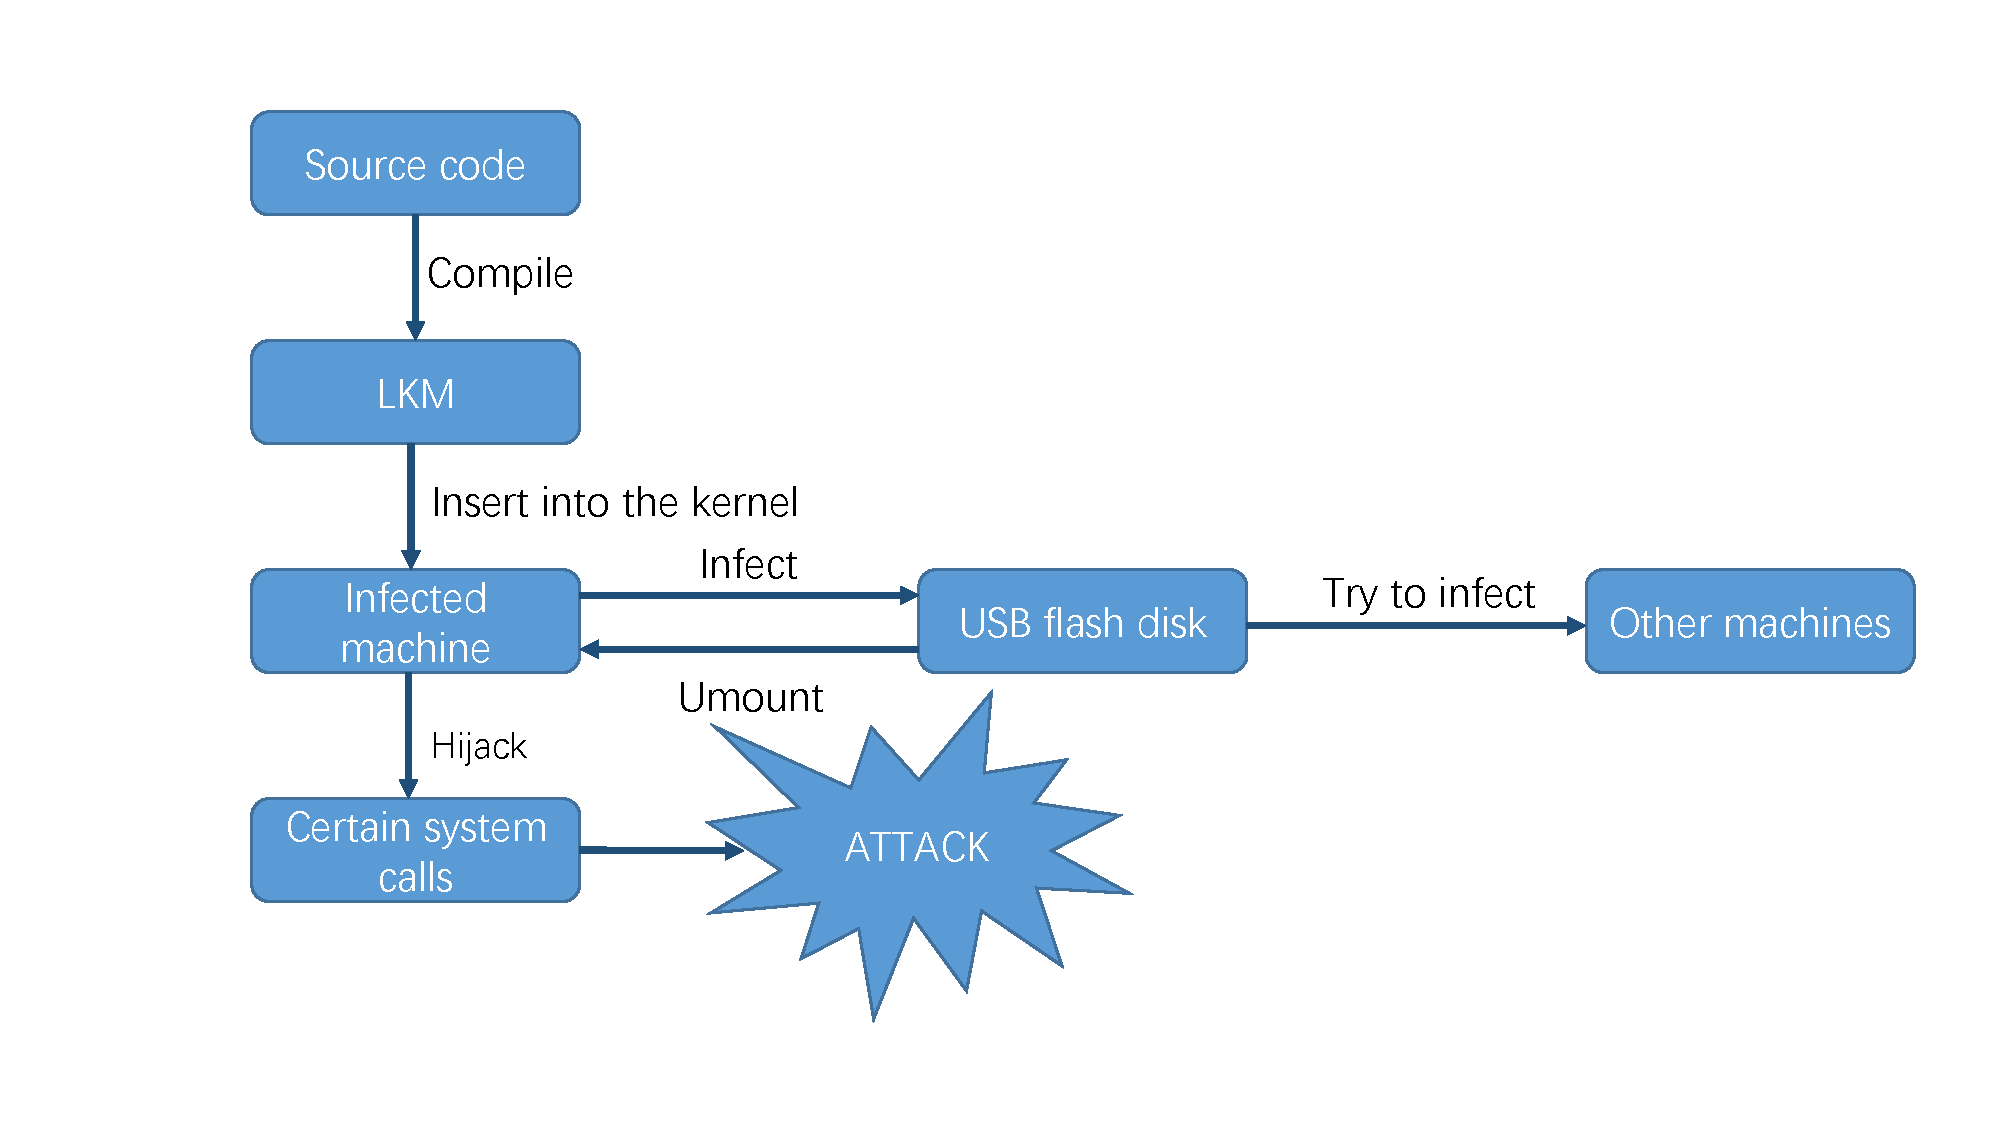
\includegraphics[width=0.5\paperwidth]{image/flowchart}
\par\end{centering}

\caption{病毒工作原理流程示意图\label{fig:=0075C5=006BD2=005DE5=004F5C=00539F=007406=006D41=007A0B=00793A=00610F=0056FE}}
\end{figure}


本文将介绍该病毒实现中的几大关键部分:
\begin{itemize}
\item 病毒的感染: 病毒如何像木马一样潜入内核, 像 rootkit 一样隐藏自己;
\item 劫持系统调用: 病毒如何对操作系统内核与用户连接的桥梁 —— ``系统调用'' 进行劫持, 以及系统调用劫持的意义;
\item 病毒的传播: 病毒如何对虚拟文件系统, 即 virtual file system (VFS) 进行随意的修改;
\item 隐藏进程: 通过系统调用的劫持, 病毒对任意一个进程实现隐藏.
\end{itemize}


本文不会包括下面内容:
\begin{itemize}
\item 全部源码: 阅读全部源码, 并不如领悟它的思想更有意义;
\item 权限提升: 尽管内核有一些漏洞, 可能的权限提升做法很多, 然而这些做法通常不具有太高的普适性, 与理论结合不够紧密;
\end{itemize}


此外, 附件包含该病毒的全部源码, 以及一个 VMWare Workstation 可以直接载入的磁盘镜像 \footnote{VMware® Workstation 12.0.0 build-2985596, Windows / Mac OS X / Ubuntu
14.04 / Ubuntu 15.04 下均测试可行}, 用以验证实验.

\newpage{}


\chapter{病毒的感染}



\vspace*{2cm}

\textit{However, as every parent of a small child knows, converting
a large object into small fragments is considerably easier than the
reverse process.}

\begin{flushright}
—— Andrew S. Tanenbaum
\par\end{flushright}

\newpage{}


\section{可装载内核模块}



可加载内核模块 (loadable kernel module, 即 LKM) 是包含在操作系统运行期间向内核添加扩展代码的目标文件.

LKM 主要用于在系统内核中随时为新增的设备驱动、文件系统驱动、系统调用提供支持, 而当一个模块的功能不再需要时, 则可以随时卸载以释放存储空间以及其他系统资源.
Linux内核采用的就是这种模块化的结构, 允许向运行中的内核动态插入和删除代码段, 从而并不需要在运行前把所有可能会用到的功能都编译进内核中,
导致浪费大量的内存存放暂时或很长一段时间内都用不到的功能, 也不需要每次增加新的功能或卸载不再使用的功能时用户都得重新编译和运行内核.
 

尽管这种机制为用户和系统内核之间的交互增加了灵活性和极大的便捷, 但LKM是内核的一部分, 轻易改写内核也增大了系统崩溃的概率. 另外,
静态内核占用的是一段连续的内存空间, 而LKM则会使内核在存储上变得不连续、碎片化, 这会导致实际运行效果上产生一些微小的性能降低.

LKM病毒利用模块技术作为操作系统内核的一部分运行, 通过劫持系统调用几乎可以完成隐藏、发作等所有功能, 比传统hacking技术更加强大更加不易被发觉.

我们的病毒即使用LKM实现. 该病毒拥有木马的特性: 一旦用户以 root 权限执行被感染的文件, 该病毒就会作为 LKM 自动插入到系统中.


\section{在 LKM 中隐藏自身}



为了任务的调度, 一个多任务操作系统一定是维护了一个或者多个表, 用以维护当前运行的所有进程. 一个病毒为了不被发现, 需要在用户查看这张表的时候,
隐藏自己. 

有两种典型的方法: 第一, 将自己直接从表中删除;第二, 从系统调用的返回值中删除自己所在的项目. 

方法二的实现比较繁琐, 需要用到下面提到的系统调用挂钩(system call hooking)的技术. 为了简便, 我们采用了第一种方法. 

\begin{figure}[H]
\begin{centering}
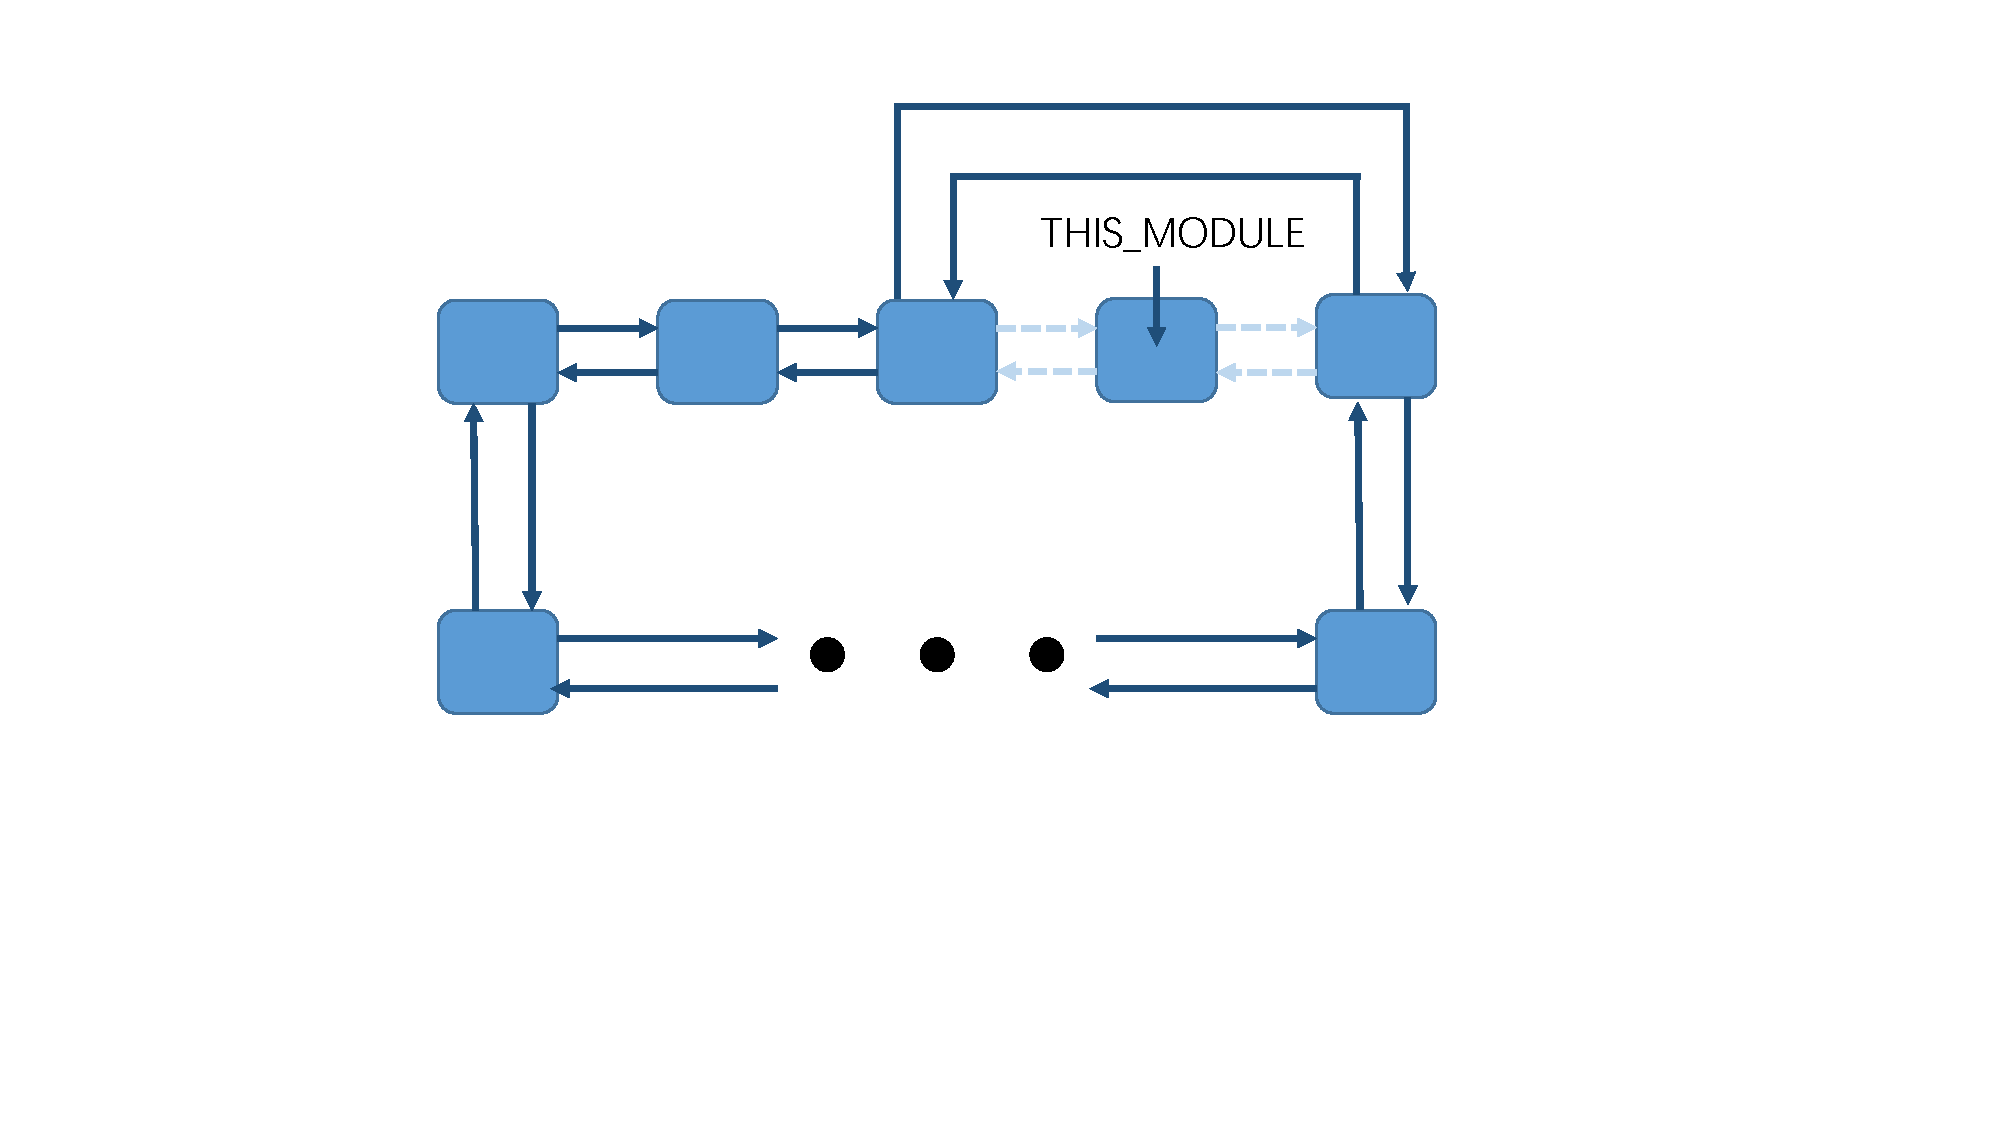
\includegraphics[width=0.5\paperwidth]{image/delete_entry}
\par\end{centering}

\caption{从双向循环链表中删除元素\label{fig:=004ECE=0053CC=005411=005FAA=0073AF=0094FE=008868=004E2D=005220=009664=005143=007D20}}
\end{figure}


对于 Linux 系统的 LKM, 我们首先需要从 \texttt{lsmod} 命令和 \texttt{/proc/modules}
中隐藏自身. 事实上, \texttt{lsmod} 和 \texttt{/proc/modules} 文件一样, 通过查看 Linux内核中的结构体
\texttt{struct module} 构成的循环链表, 来查找所有载入的模块.  如图 \ref{fig:=004ECE=0053CC=005411=005FAA=0073AF=0094FE=008868=004E2D=005220=009664=005143=007D20},
Linux 内核中, 定义了 \texttt{list\_del\_init} 函数, 能帮助我们删除双向链表中的给定元素. 直接调用该函数,
就可以达到从 \texttt{lsmod} 和 \texttt{/proc/modules} 里面隐形的目的:  



% \vspace*{0.5cm}

\begin{mdframed}[skipabove=7pt,
	skipbelow=7pt,
	rightline=false,
	leftline=true,
	topline=false,
	bottomline=false,
	linecolor=gray,
	backgroundcolor=black!5,
	innerleftmargin=5pt,
	innerrightmargin=5pt,
	innertopmargin=-4pt,
	innerbottommargin=-12pt,
	leftmargin=0cm,
	rightmargin=0cm,
	linewidth=4pt]
\begin{lstlisting}[language=C]
list_del_init(&THIS_MODULE->list);
`
\end{lstlisting}
\end{mdframed}

% \vspace*{0.5cm}



除此之外,  Linux 内核中还维护了一个叫做 sysfs 的模块, 以虚拟文件系统的形式, 显示出内核中的子系统、硬件设备和相关的驱动程序.
我们的 LKM 便在其中. 用户可以通过查看 \texttt{/sys/module/} 来获知哪些模块在运行. 我们需要从 sysfs
中删除掉我们的模块来实现进一步隐藏. 幸运的是,  sysfs 中的模块也是由链表串在一起, 我们只需要找到相关的链表, 并进行删除操作即可.
具体代码也只有一行: 



% \vspace*{0.5cm}

\begin{mdframed}[skipabove=7pt,
	skipbelow=7pt,
	rightline=false,
	leftline=true,
	topline=false,
	bottomline=false,
	linecolor=gray,
	backgroundcolor=black!5,
	innerleftmargin=5pt,
	innerrightmargin=5pt,
	innertopmargin=-4pt,
	innerbottommargin=-12pt,
	leftmargin=0cm,
	rightmargin=0cm,
	linewidth=4pt]
\begin{lstlisting}[language=C]
kobject_del(&THIS_MODULE->mkobj.kobj);
`
\end{lstlisting}
\end{mdframed}


% \vspace*{0.5cm}



这样操作的副作用做了之后, 内核模块就不能被直接删除了, 除非我们再把该模块重新接回上述链表 —— 当然, 对于一个病毒而言, 这完全没有必要.
 

\newpage{}


\chapter{劫持系统调用}



\vspace*{2cm}

\textit{Those that can, do. Those that can't, complain.}

\begin{flushright}
—— Linus Torvalds
\par\end{flushright}

\newpage{}


\section{系统调用及其流程}



系统调用 (system call, 即 syscall) 是在用户态中运行一个程序时需要一个系统服务而在内核态执行的调用指令.

系统调用为应用程序调用硬件和其他系统资源提供了途径, 是用户态和内核态交互的接口. 当应用程序需要读写文件时, 通过系统调用提供的抽象硬件接口,
就不需要考虑实际文件所在的磁盘类型、文件系统等问题. 同时, 系统调用使得内核可以决定调用权限, 以防止应用程序非法使用硬件设备,
占用其它进程资源, 或对系统造成破坏等不良行为, 从而保障系统安全和稳定. 另外, 系统调用也使得多任务处理和虚拟内存的实现成为可能,
便于进程管理.

\begin{figure}[H]
\begin{centering}
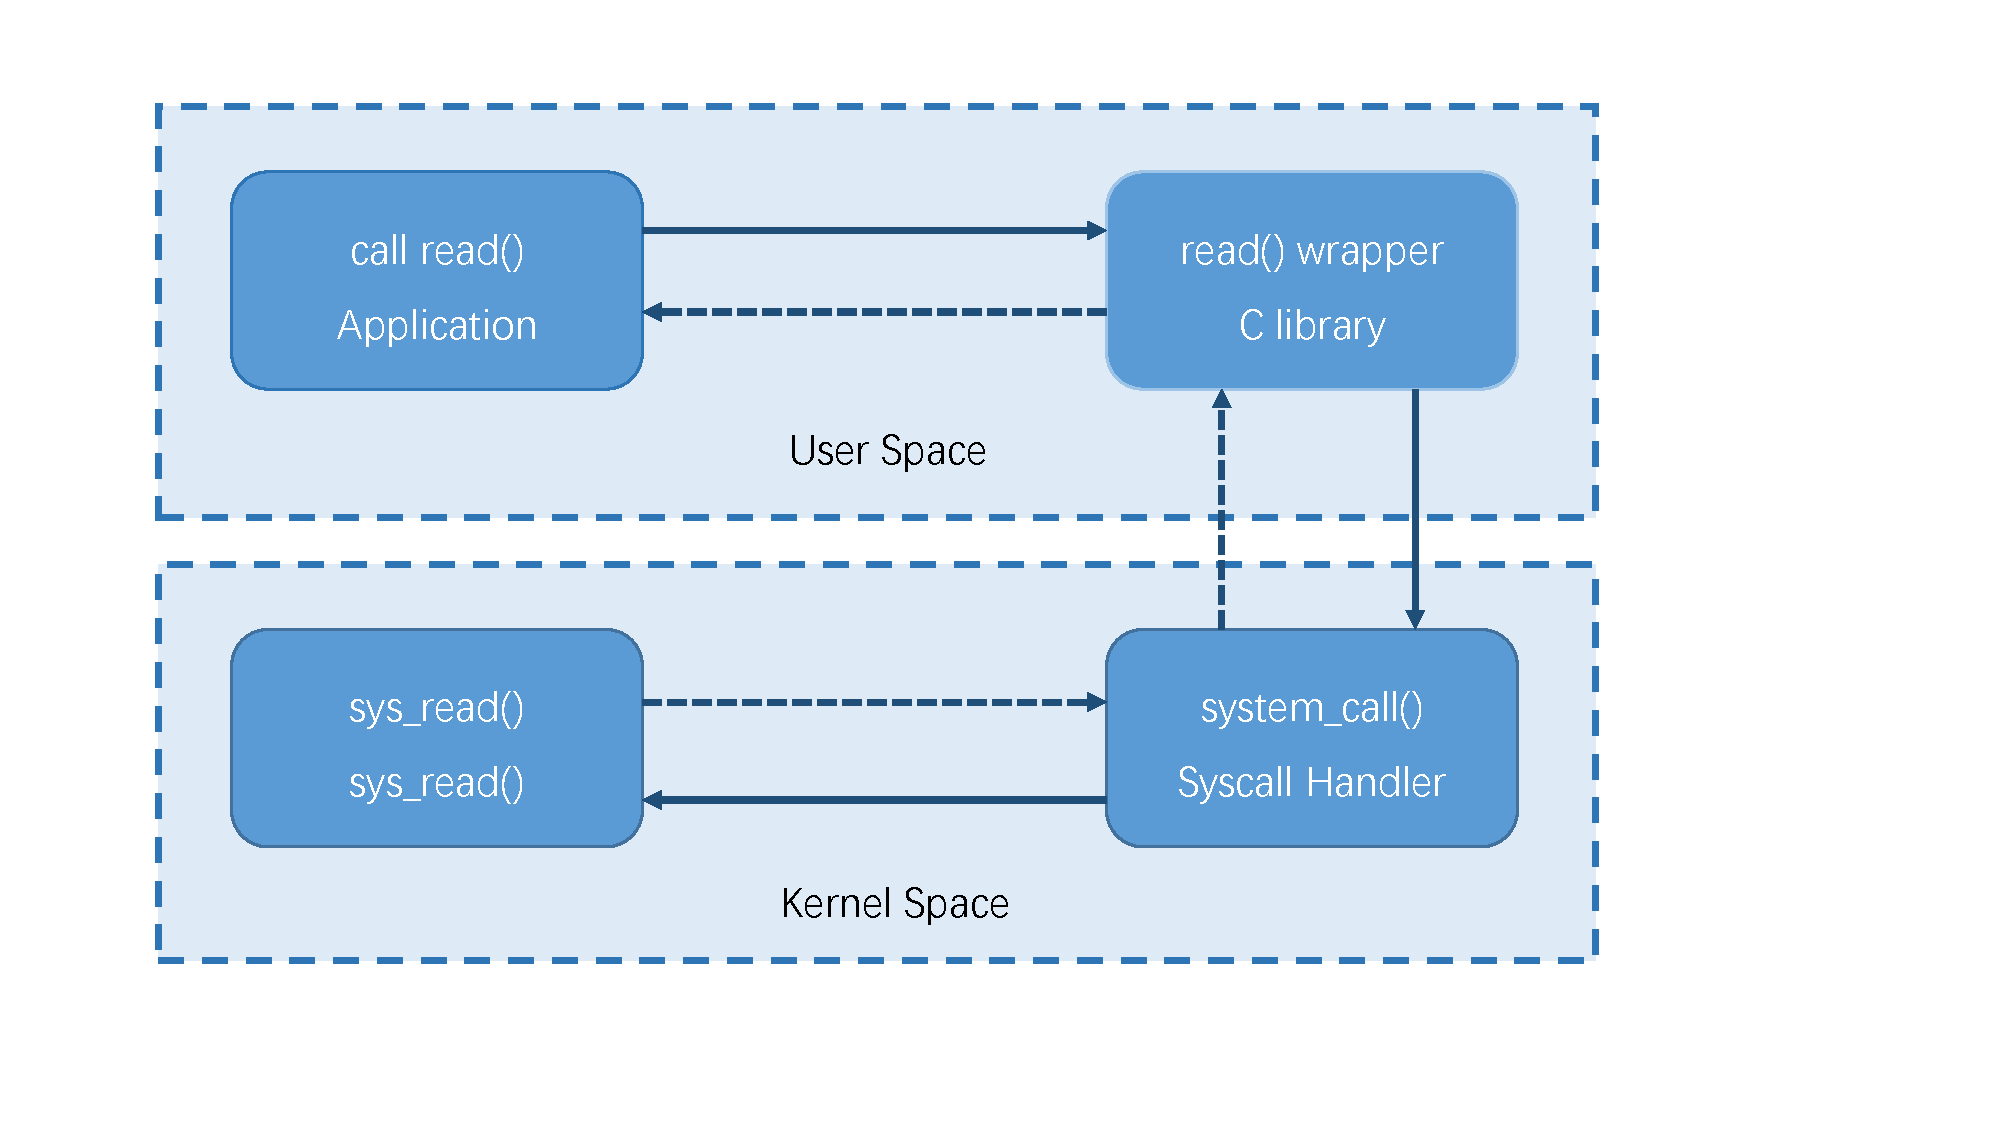
\includegraphics[width=0.5\paperwidth]{image/syscall}
\par\end{centering}

\caption{系统调用的流程: 以 read 为例}


\end{figure}


在Linux中, 每一个系统调用都被分配一个唯一的编号, 称作 syscall number. 记录这个对应的系统调用列表就存储在内核中的名叫
sys\_call\_table 的系统调用表中. 

当一个用户态进程执行系统调用, 会通过 syscall number 而非名称用来确定具体是哪一个系统调用被执行. syscall
number 一旦确定就不可更改, 否则编译好的应用程序会崩溃; 移除的系统调用的 syscall number 也不可再用于其它系统调用,
否则先前编译好的应用程序运行时会执行其它的系统调用.

系统调用流程分为如下四个步骤:
\begin{enumerate}
\item 触发系统调用处理程序 (system call handler) 陷入内核态;
\item 系统调用处理程序从特定寄存器上读取 syscall number 以及其它调用参数;
\item 执行相应的系统调用;
\item 返回至用户态.
\end{enumerate}


内核代码存于一段受保护的内存空间中, 所以用户态的应用程序不能直接通过过程调用执行内核中的程序. 于是, 用户态的应用程序需要一个软中断向内核发出信号,
即抛出一个异常让系统切换至内核态去执行异常处理程序, 也就是系统调用处理程序 (system call handler) . 以 x86
为例: x86 处理器上的软中断是指令 int \$0x80, 这个中断指令会导致系统切换至内核态并且执行系统调用处理程序 exception
vector 128. 这个系统调用处理程序就被命名为函数 system\_call(), 用汇编语言实现.

仅仅进入内核是显然不够的, 用户程序需要告诉内核要执行哪一个系统调用, 所以必须将 syscall number 传给内核. x86
上 syscall number 是通过寄存器 eax 传给内核的, 在系统陷入内核态之前用户态会先将 syscall number
存在寄存器 eax 上, 系统调用处理程序执行时会从 eax 上读取 syscall number. 函数system\_call()会检查
syscall number 的合法性, 没有问题的话就执行相应的系统调用 call {*}sys\_call\_table(,\%eax,4).
系统调用执行结束以后即返回用户态, 并通过寄存器eax传递返回值. 


\section{Hooking 与 Ring}



挂钩 (hooking) 是涵盖了通过监控软件组件之间的过程调用、信息传递或事件的方式更改或扩展操作系统、应用程序或其他软件组件的行为的一系列技术.
处理这些被监控的过程调用、信息传递或事件的代码即是钩子 (hook). Hooking 可以用来排除错误或扩展功能, 例如在键盘或鼠标发送的信号到达应用程序之前监视键盘或鼠标的事件信息,
或监视系统调用, 以控制和调整应用程序及其组件的功能实现; hooking 也被广泛应用于标准检查程序中, 例如 3D 游戏中帧频的计量,
其输入输出就是通过 hooking 实现的. 另一方面, hooking也会被应用在恶意程序中, 例如 rootkit 会通过 hooking
技术伪造 API 调用的输出结果以隐匿自己, wallhack 则通过监控游戏中的过程调用并篡改玩家看到的信息使一方获益. 我们的病毒就是通过
hooking 劫持系统调用实现的. 

\begin{figure}[H]
\begin{centering}
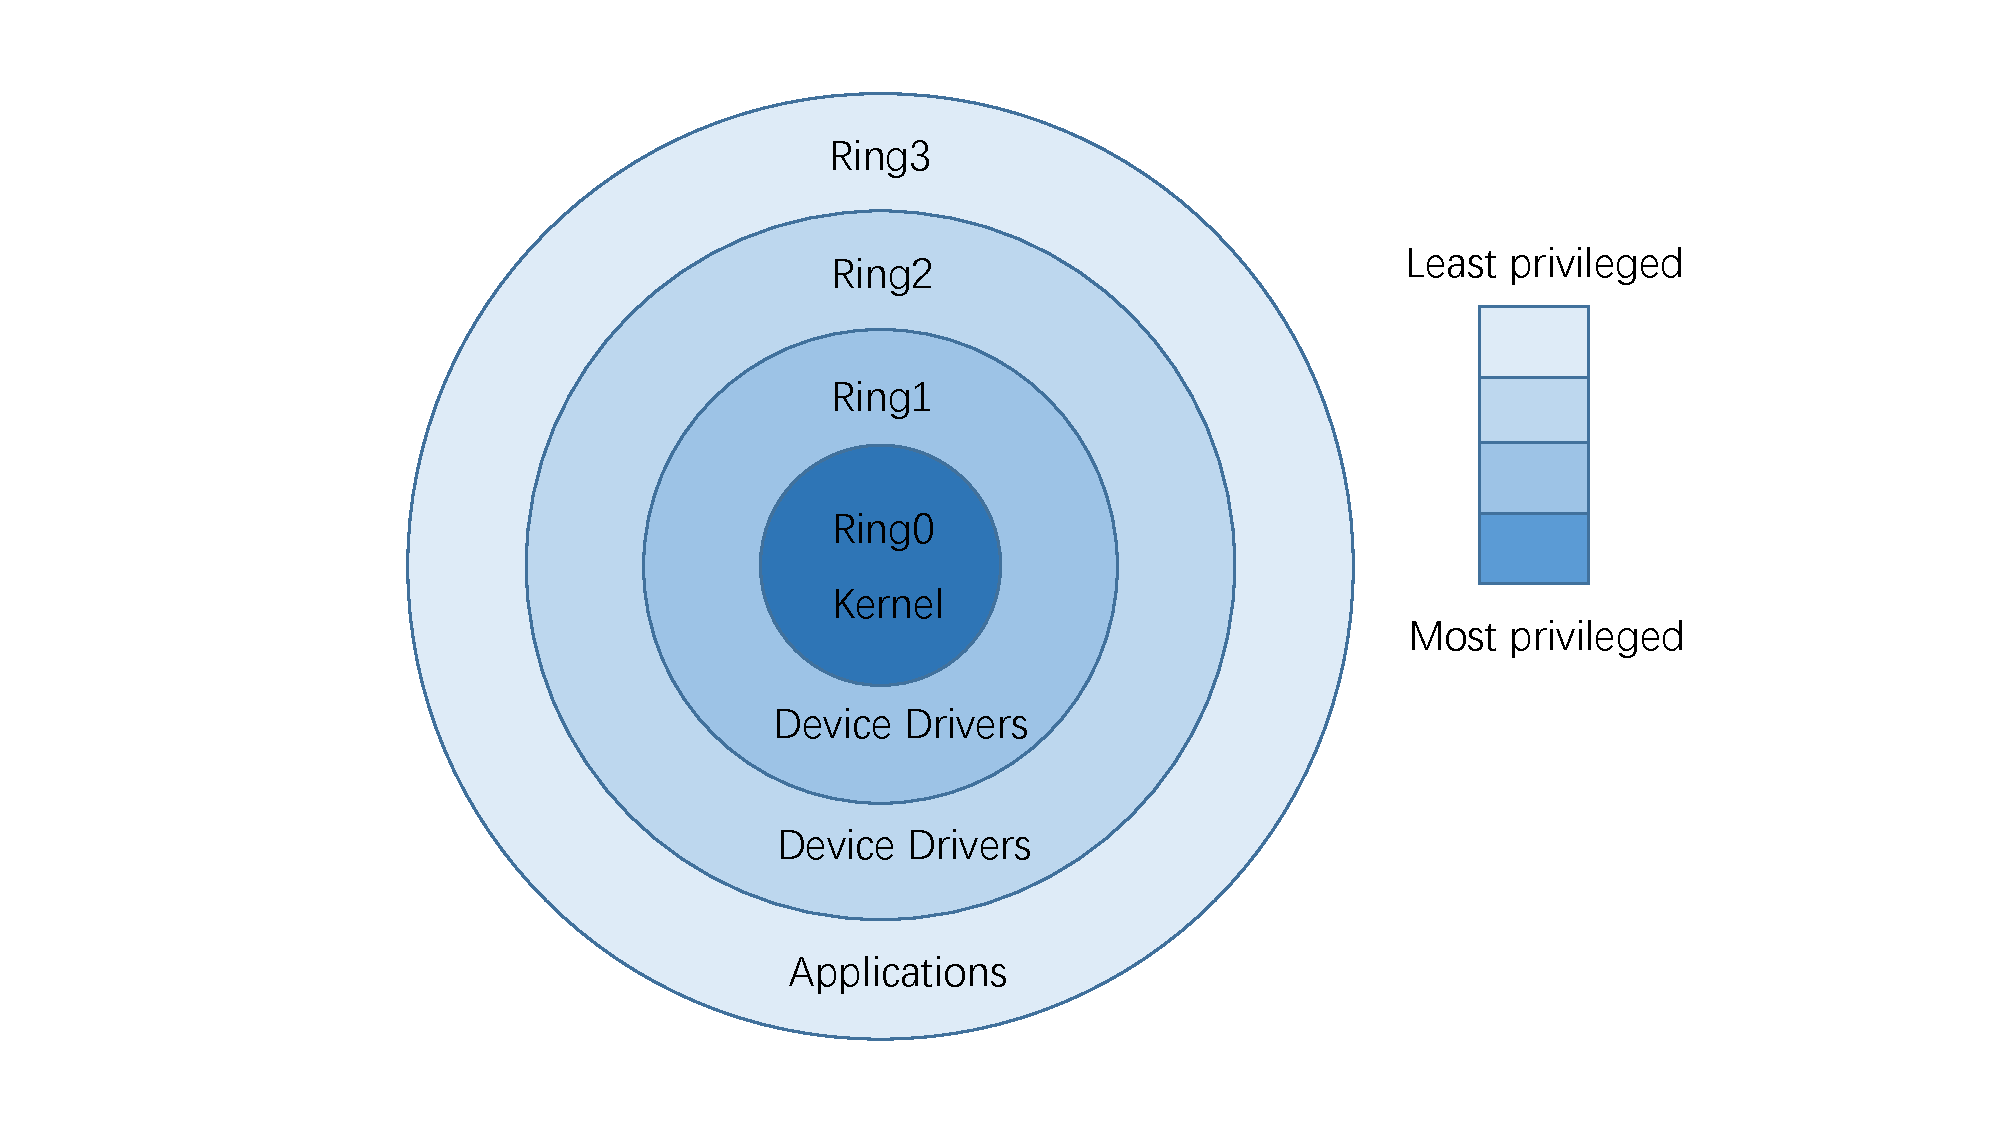
\includegraphics[width=0.5\paperwidth]{image/ring}
\par\end{centering}

\caption{Ring 结构示意图\label{fig:Ring-=007ED3=006784=00793A=00610F=0056FE}}


\end{figure}


如图 \ref{fig:Ring-=007ED3=006784=00793A=00610F=0056FE}, 保护环 (protection
ring) 是保护数据及功能不受运行错误和恶意攻击影响的机制, 操作系统提供了访问资源时不同级别的权限, 一个保护环即是计算机体系结构中的一个权限等级,
等级编号越小, 信任度越高. 大部分操作系统中, ring0 是权限最高等级, 相当于内核态, 可以直接与 CPU、内存等硬件交互;
ring3 是普通应用程序等级, 相当于用户态. 外层权限低的环通过预定义方式经由特殊的门访问内层环的资源, 这样可以避免低级别的程序误用高级别的资源而带来的安全问题,
例如在 ring3 上运行的监控程序在用户没有知晓的情况下企图打开摄像头就会被阻止, 因为相应的硬件启用权限是 ring1 级别的.
尽管保护环提高了系统安全性, 但是环的等级不会无休止地细分下去, 因为不同的层次的环之间的切换会造成大量的性能损失, 降低运行效率.
2.6 版本的 Linux 内核仅仅使用了两个权限等级, 分别是 ring0 对应的内核态和 ring3 对应的用户态. 大约有 15
条机器指令被 CPU 严格限制在 ring0 层, 主要保护内存、I / O 端口等资源. 一旦在 ring3 用户态调用这些指令,
系统就会抛出异常 —— 这与操作系统账户权限无关, 无论是 root、guest 还是 regular user, 所有用户态程序都是在
ring3 层上运行, 内核代码都是在 ring0 层上运行, 两者之间通过系统调用切换. 简而言之, 系统调用就是他们之间的桥梁.

我们的病毒, 经过反复尝试, 最终确定了适应性最好的 ring0 hooking, 对系统调用进行劫持.


\section{系统调用的挂钩}



\begin{figure}
\begin{centering}
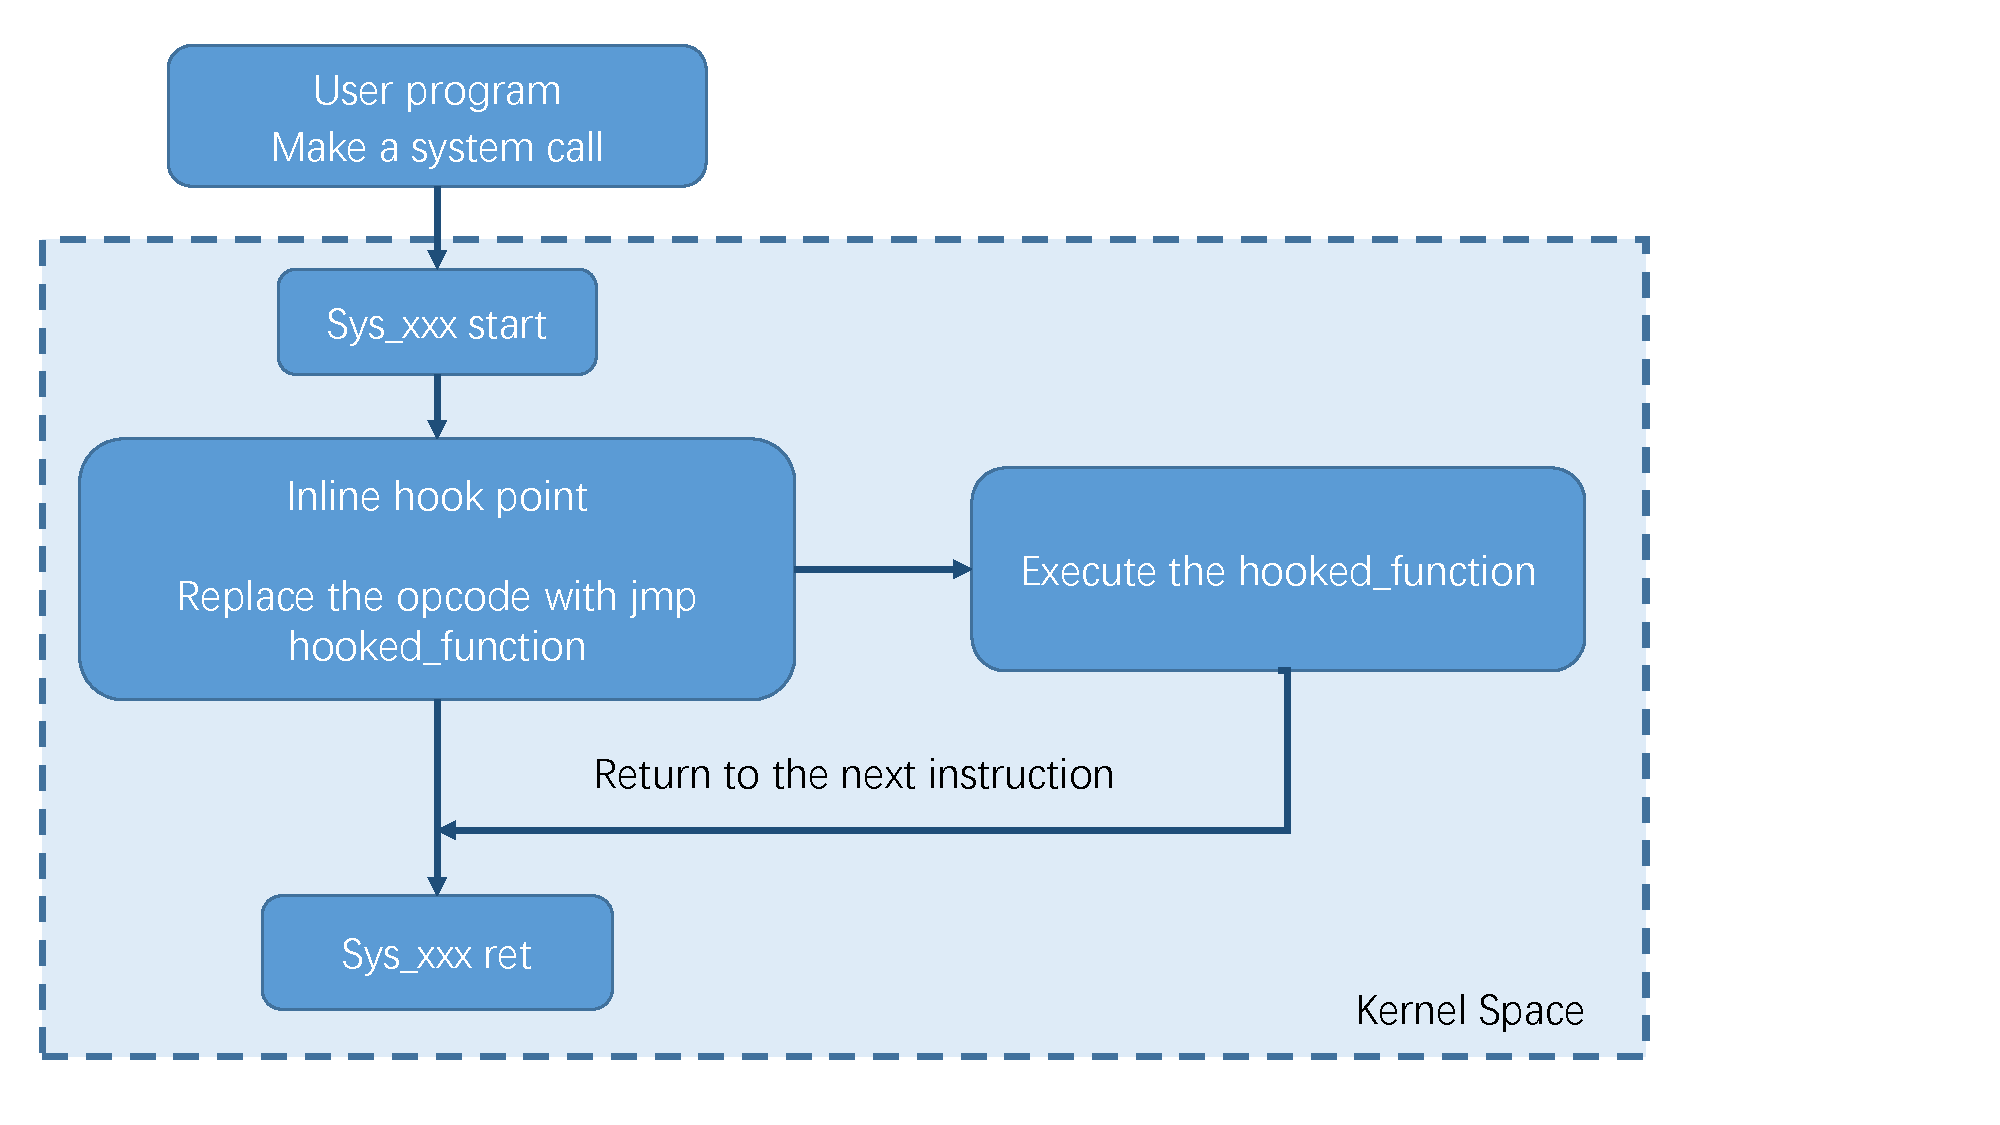
\includegraphics[width=0.4\paperwidth]{image/syscall_hooking}
\par\end{centering}

\caption{系统调用劫持\label{fig:=007CFB=007EDF=008C03=007528=0052AB=006301}}
\end{figure}


如果一个病毒, 处于内核态, 并能够自由修改、劫持系统调用, 而不被杀死, 那么这个病毒几乎能掌控操作系统的一切: 能随意删改文件系统,
能随意向进程发送信号, 能随意开启或关闭系统中断, 甚至能随意分发 root 权限. 因此, 对于系统调用的劫持, 是我们工作的重点.

如图 \ref{fig:=007CFB=007EDF=008C03=007528=0052AB=006301}, 通常劫持一个系统调用的流程如下:
\begin{enumerate}
\item 找到需要劫持的系统调用在系统内核数组中的入口位置;
\item 保存内核中原来的调用函数对应的指针sys\_call\_table{[}id{]};
\item 用我们重新编写的函数指针替换给sys\_call\_table{[}id{]}.
\end{enumerate}


第一步通常比较容易, 而一些在 32 位 2.4 内核中的做法, 在 64 位的 2.6 内核中已经失效. 我们尝试了下面许多方案:

第一种做法, 直接从 \texttt{/boot/System.map{*}} 文件里面寻找 \texttt{sys\_call\_table}
变量, 这就是系统调用表的确切位置所在, 并不会随时间改变. 因此, 我们把这个变量作为常量存入我们的病毒中. 然而, 这样做的普适性不会很强,
对于不同的内核子版本, 系统调用表的地址可能会不一样.  

第二种做法, 通过 0x80, 即系统中断的处理程序, 从其中的内存空间里面找出系统调用表的位置. 具体步骤是, 获取中断描述表 (IDT)
的地址, 通过简单的地址偏移, 找出中断的处理程序的内存空间, 从中获取系统调用表的地址. 这个做法依赖于中断描述表, 而且需要一些对于操作系统架构的假设,
因此我们最终也没有采用这种做法. 

第三种做法, 通过 Linux 新增的安全模块 (linux security module, LSM) 进行挂钩. 事实上有些内核版本的
LSM 并不安全. 通过图 \ref{fig:LSM-Hooking} 中的流程, 可以轻松劫持系统调用. 我们认为该做法不具有普适性,
没有采用这种方法.

\begin{figure}[H]
\begin{centering}
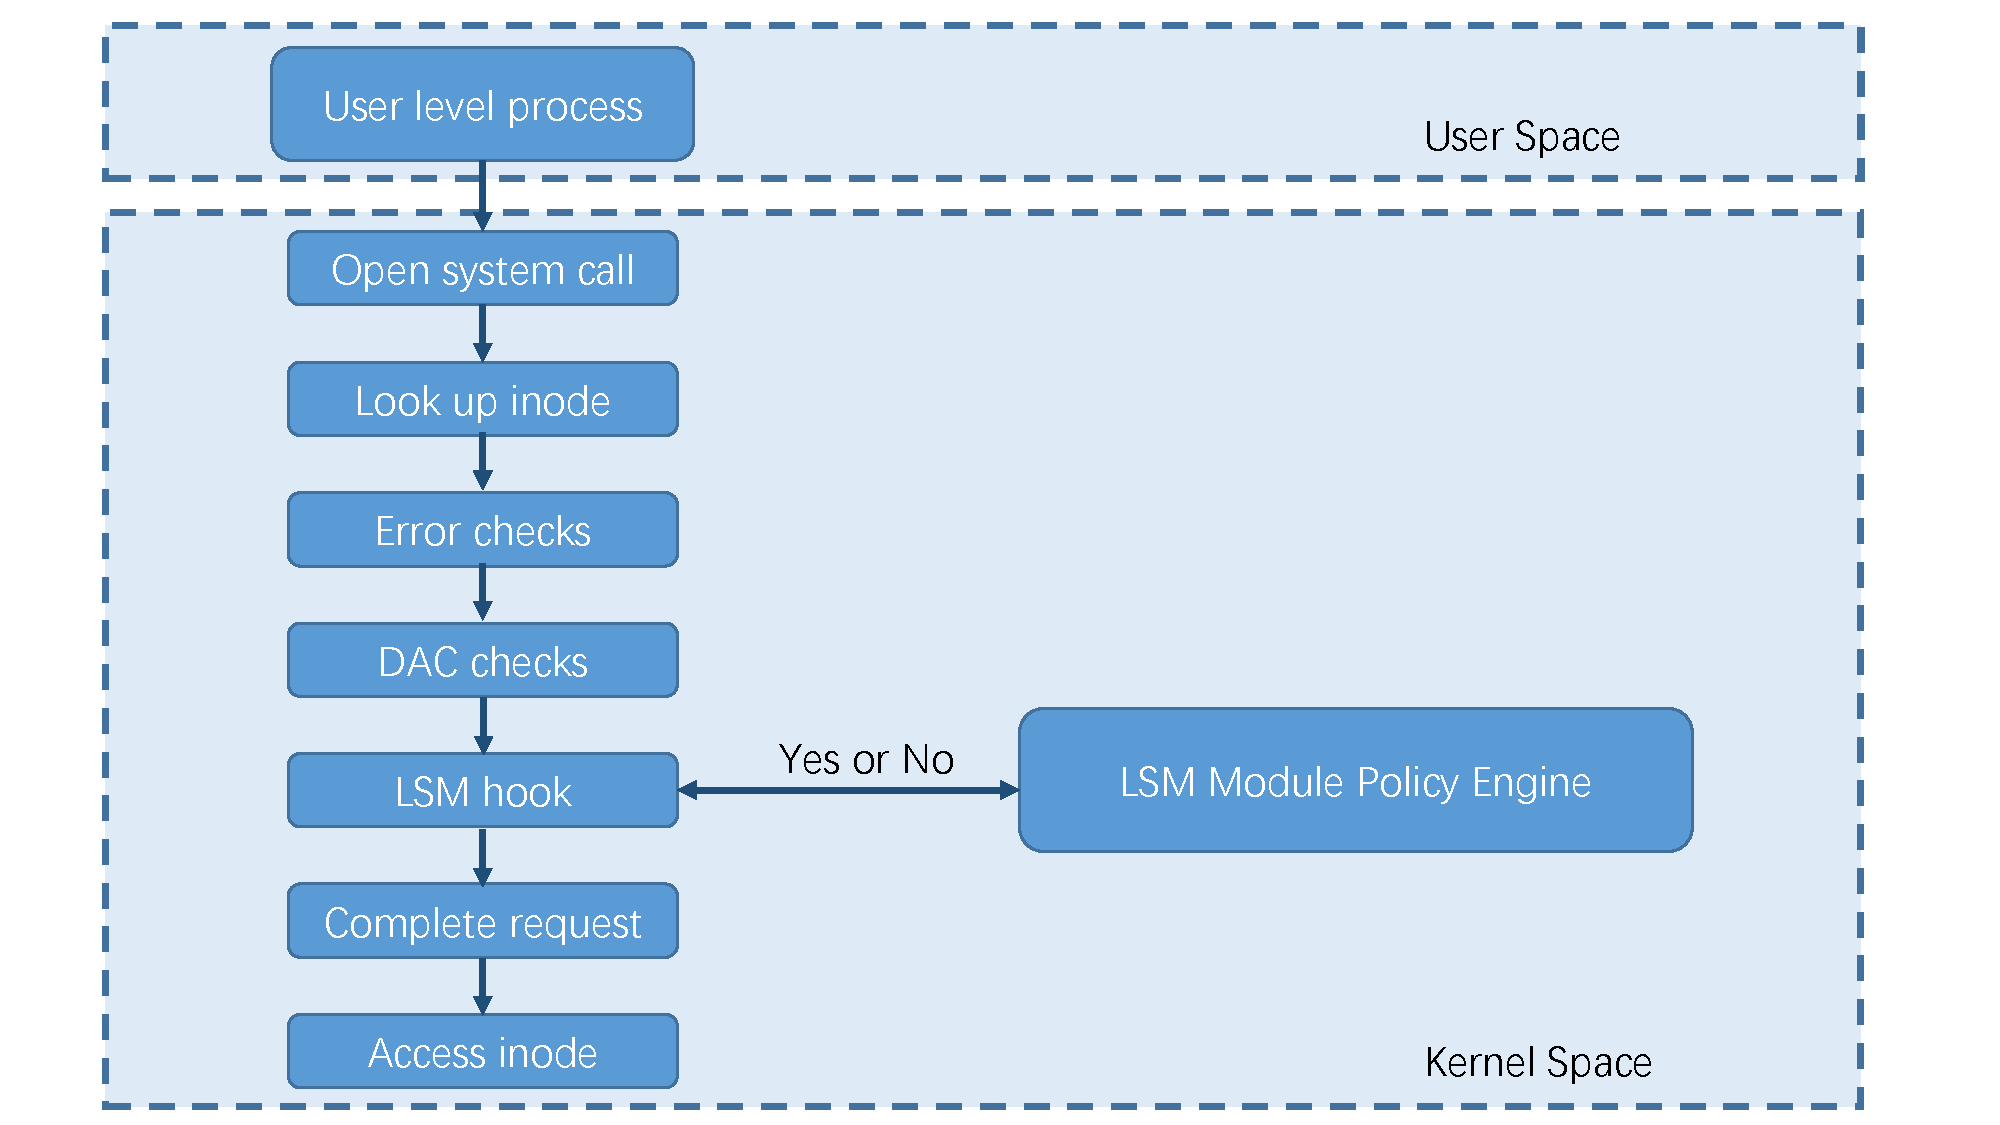
\includegraphics[width=0.5\paperwidth]{image/lsm_hooking}
\par\end{centering}

\caption{LSM Hooking\label{fig:LSM-Hooking}}
\end{figure}


第四种做法, 也是最有效的一种做法: 首先可以确定系统调用表一定在一段给定的地址空间内, Linux 的内核设计保证了系统调用表一定落在一个内存区间中,
我们通过对内存区间的顺序搜索, 就可以找到系统调用表. 

对于 2.4 版本的内核, 第二步是简单的. 然而到了 2.6 版本, 找到系统调用表之后, 如果我们直接写系统调用表, 以完成我们的挂钩工作,
我们的病毒会被操作系统发现并杀死. 其中的原因是, 为了防止对系统调用表的修改, 系统调用表所在的页表被设置为只读的. 因此我们需要对这个页表加入可写权限.
这时候, 我们需要修改 cr0 寄存器. 对于不同的系统架构, 写保护位是不一样的: 对于 64 位系统, 写保护位则是第 20 位.
我们写了一段汇编, 修改这个寄存器, 之后的替换工作就变得简单. 汇编代码如下:

% \vspace*{0.5cm}

\begin{mdframed}[skipabove=7pt,
	skipbelow=7pt,
	rightline=false,
	leftline=true,
	topline=false,
	bottomline=false,
	linecolor=gray,
	backgroundcolor=black!5,
	innerleftmargin=5pt,
	innerrightmargin=5pt,
	innertopmargin=-4pt,
	innerbottommargin=-12pt,
	leftmargin=0cm,
	rightmargin=0cm,
	linewidth=4pt]
\begin{lstlisting}[language=C]
unsigned long long clear_write_protect_bit_of_cr0(void) {
	unsigned long long cr0 = 0;
	unsigned long long ret;

	asm volatile("movq %%cr0, %0": "=a"(cr0));
	ret = cr0;
	cr0 &= ~0x10000LL; // `clear the 20-th bit of CR0`
	asm volatile ("movq %0, %%cr0": : "a"(cr0)); 
	return ret; 
}
`
\end{lstlisting}
\end{mdframed}


% \vspace*{0.5cm}

\newpage{}


\chapter{病毒的传播与虚拟文件系统}



\vspace*{2cm}

\textit{One of my most productive days was throwing away 1,000 lines
of code.}

\begin{flushright}
—— Ken Thompson
\par\end{flushright}

\newpage{}


\section{虚拟文件系统简介}



虚拟文件系统 (virtual file system, 即 VFS) 是在用户进程和实际文件系统之间的抽象层, 为不同类型的实际文件系统提供统一的访问方式,
使得应用程序通过虚拟文件系统调用底层的实际文件系统来具体管理数据, 而不必知道数据确切存储在什么位置或者是什么样的文件系统. 所有和文件相关的系统调用在最初的处理上都指向虚拟文件系统,
这些调用都是标准的POSIX系统调用, 所以虚拟文件系统向上对用户进程的接口是POSIX接口; 为使每一个文件系统完成功能调用, 虚拟文件系统向下对实际文件系统有
VFS 接口, 每当增加一个新的文件系统, 就必须确定它包含接口需要的所有功能调用, 并在注册时向VFS提供这样的函数地址列表. 图\ref{fig:=00865A=0062DF=006587=004EF6=007CFB=007EDF=007B80=0056FE}
给出了 VFS 的实现逻辑.

\begin{figure}[H]
\begin{centering}
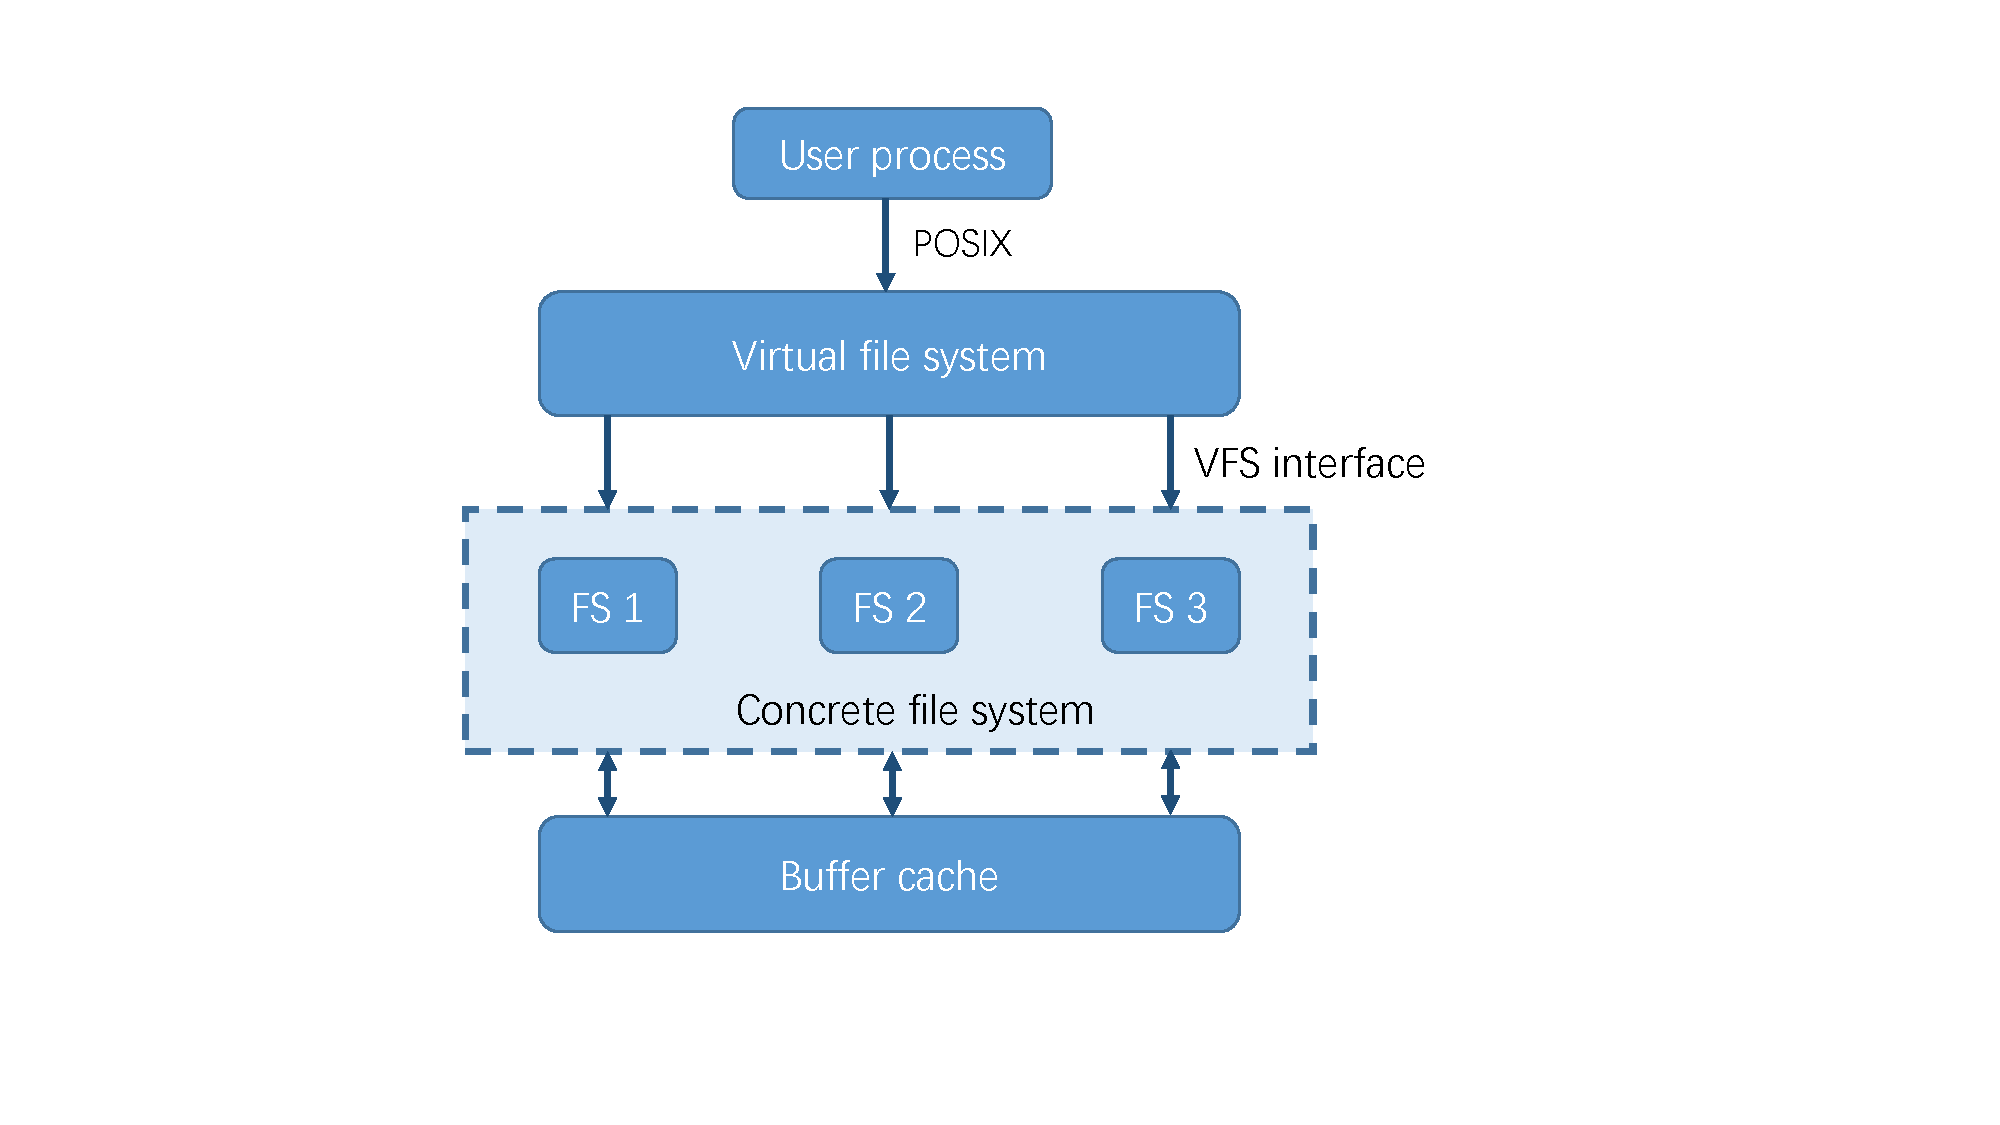
\includegraphics[width=0.5\paperwidth]{image/vfs}
\par\end{centering}

\caption{虚拟文件系统简图\label{fig:=00865A=0062DF=006587=004EF6=007CFB=007EDF=007B80=0056FE}}


\end{figure}


调用一个装载好的文件系统的流程如下:
\begin{enumerate}
\item 解析路径, 通过搜索已装载文件的超块表确定该文件系统的超块;
\item 创建一个 v-node 并调用实际文件系统, 将所有文件 i-node 中的信息以及指向功能表的指针复制到 v-node 中;
\item 在文件描述符表中为调用进程创建一个入口, 并向调用者返回文件描述符;
\item 当进程用文件描述符调用具体操作时, VFS 通过进程表、文件描述符表找到 v-node, 并跟随指针指向功能表调用处理相应操作的功能,
最后在实际文件系统中实现功能调用. 
\end{enumerate}

\section{伪装成用户态}



事实上, 在工业上和开源项目中, 在Linux内核里面进行文件操作是不被鼓励的. 这会大大降低一个模块的安全性和灵活性. 这意味着,
如果内核和一个绝对路径有关的文件进行交互, 那么在版本更迭的时候这个路径要被保留, 或者所有使用这个路径的内核都要重写. 而同时,
如果这个文件被用户找到, 并且用 root 权限进行了修改, 那么用户就可以直接通过修改这个文件来干预内核态的工作, 这都不符合 Linux
的设计理念.  

我们的实现方式, 主要依赖于虚拟文件系统提供给我们的 \texttt{vfs\_read} 和 \texttt{vfs\_write}
接口进行读写. 这些功能本质上都是利用系统调用实现的, 而系统调用都是由用户态发出的, 虽然我们身处内核内核态的权限高于用户态, 但是还有一个重要的区别在于,
内核态的缓冲区和用户态的缓冲区分处于两地. 当我们进行文件 I / O 的系统调用的时候, 这些系统调用会检查我们所处的数据段边界,
所以在进行 I / O 操作的时候要通过替换缓冲区段将自己伪装成用户态. 可以通过如下代码段实现:

% \vspace*{0.5cm}

\begin{mdframed}[skipabove=7pt,
	skipbelow=7pt,
	rightline=false,
	leftline=true,
	topline=false,
	bottomline=false,
	linecolor=gray,
	backgroundcolor=black!5,
	innerleftmargin=5pt,
	innerrightmargin=5pt,
	innertopmargin=-4pt,
	innerbottommargin=-12pt,
	leftmargin=0cm,
	rightmargin=0cm,
	linewidth=4pt]
\begin{lstlisting}[language=C]
void enter_usr_space(void) {
	old_fs = get_fs();
	set_fs(get_ds());
}
`
\end{lstlisting}
\end{mdframed}

% \vspace*{0.5cm}

其中 \texttt{old\_fs} 为了回复到原缓冲区段而记录下的临时变量, 是一个全局变量. 有了上面这段代码, 当离开用户态的缓冲区段时候的代码也就呼之欲出了,
只要将缓冲区段重新设回原来的区段即可:

% \vspace*{0.5cm}

\begin{mdframed}[skipabove=7pt,
	skipbelow=7pt,
	rightline=false,
	leftline=true,
	topline=false,
	bottomline=false,
	linecolor=gray,
	backgroundcolor=black!5,
	innerleftmargin=5pt,
	innerrightmargin=5pt,
	innertopmargin=-4pt,
	innerbottommargin=-12pt,
	leftmargin=0cm,
	rightmargin=0cm,
	linewidth=4pt]
\begin{lstlisting}[language=C]
void quit_usr_space(void) {
	set_fs(old_fs);
}
`
\end{lstlisting}
\end{mdframed}


% \vspace*{0.5cm}


\section{文件打开}



在 Linux 内核中有类似于 C 风格的 \texttt{freopen} / \texttt{fopen} 的 \texttt{filp\_open},
惟一的不同是对于行为的指定的要求更加明确, 因为内核里面所作的事情更加的底层. \texttt{filp\_open(char {*},
int, int)} 第一参数为函数的路径, 第二个参数为打开文件的权限, 第三个参数为打开操作为一个创建操作的时候, 创建出来的文件的权限. 

% \vspace*{0.5cm}

\begin{mdframed}[skipabove=7pt,
	skipbelow=7pt,
	rightline=false,
	leftline=true,
	topline=false,
	bottomline=false,
	linecolor=gray,
	backgroundcolor=black!5,
	innerleftmargin=5pt,
	innerrightmargin=5pt,
	innertopmargin=-4pt,
	innerbottommargin=-12pt,
	leftmargin=0cm,
	rightmargin=0cm,
	linewidth=4pt]
\begin{lstlisting}[language=C]
struct file *reading_file_open(char *name) { 
	struct file *res;
	enter_usr_space();
	res = filp_open(name, O_RDONLY, 0);
	set_fs(old_fs);
	if (IS_ERR(res)) {
		return NULL;
	}
	quit_usr_space();
	return res;
}
`
\end{lstlisting}
\end{mdframed}


% \vspace*{0.5cm}

其中 \texttt{O\_RDONLY} 就是以只读权限打开指定文件, 打开一个现存的文件不存在权限问题, 所以最后一维用 $0$
补齐. 

% \vspace*{0.5cm}

\begin{mdframed}[skipabove=7pt,
	skipbelow=7pt,
	rightline=false,
	leftline=true,
	topline=false,
	bottomline=false,
	linecolor=gray,
	backgroundcolor=black!5,
	innerleftmargin=5pt,
	innerrightmargin=5pt,
	innertopmargin=-4pt,
	innerbottommargin=-12pt,
	leftmargin=0cm,
	rightmargin=0cm,
	linewidth=4pt]
\begin{lstlisting}[language=C]
struct file *writing_file_open(char *name) { 
	struct file *res; 
	old_fs = get_fs(); 
	set_fs(get_ds()); 
	res = filp_open(name, O_WRONLY | O_CREAT, 0644); 
	set_fs(old_fs); 
	if (IS_ERR(res)) { 
		return NULL; 
	} 
	return res; 
}
`
\end{lstlisting}
\end{mdframed}


% \vspace*{0.5cm}

打开一个文件的操作稍微复杂一点, 要以 ``读或者创建'' 的模式打开, 因为存在创建的问题需要规定其读写的权限, 最后一维的 $0644$
表示对于用户组和用户本人具备读写权限. 值得一提的是, 打开文件的模式标示符使用 $\vert$(按位或)连接二进制位上的 $1$
越多模式越灵活, 而创建文件权限的标示符用 $+$ (代数和)连接, 数字越大表示权限越严格. 


\section{文件读入}



读入文件的接口由 \texttt{struct file} 的 \texttt{f\_op} 域成员 \texttt{read(struct
file {*}, char {*}, int, loff\_t {*})} 来提供. 因为 C 还尚不支持如 C++ / Java
那样成熟的面向对象机制, 所以第一维依然要将目标文件传入, 第二维传入将结果返回的缓冲区, 第三维是读入的字节数, 第四维告诉函数从哪个字节开始读,
因为这个东西读完了会被向后挪动, 所以传入一个指针, \texttt{loff\_t} 是一个依赖于机器环境的整形变量, 由机器字宽决定
32 位或 64 位. 在我们的工作中, 封装如下: 

% \vspace*{0.5cm}

\begin{mdframed}[skipabove=7pt,
	skipbelow=7pt,
	rightline=false,
	leftline=true,
	topline=false,
	bottomline=false,
	linecolor=gray,
	backgroundcolor=black!5,
	innerleftmargin=5pt,
	innerrightmargin=5pt,
	innertopmargin=-4pt,
	innerbottommargin=-12pt,
	leftmargin=0cm,
	rightmargin=0cm,
	linewidth=4pt]
\begin{lstlisting}[language=C]
void read_file(struct file *file, char *res, int size, loff_t offset) {
	int i;
	for (i = 0; i < size; ++i) {
		res[i] = 0;
	}
	enter_usr_space();
	file->f_op->read(file, res, size, &offset);
	quit_usr_space();
}
`
\end{lstlisting}
\end{mdframed}


% \vspace*{0.5cm}


\section{文件写入}



写入的参数和读差不多, 但是使用的是虚拟文件系统提供的写接口, \texttt{int vfs\_write(struct file
{*}, loff\_t {*}, char {*}, int)} 的第一个参数是写入的文件指针, 第二个是从哪一个字节后面开始写入,
第三个从这个 buffer 开始写, 写入第四个参数表示这个 buffer 的长度. 在我们的工程中, 封装如下: 

% \vspace*{0.5cm}

\begin{mdframed}[skipabove=7pt,
	skipbelow=7pt,
	rightline=false,
	leftline=true,
	topline=false,
	bottomline=false,
	linecolor=gray,
	backgroundcolor=black!5,
	innerleftmargin=5pt,
	innerrightmargin=5pt,
	innertopmargin=-4pt,
	innerbottommargin=-12pt,
	leftmargin=0cm,
	rightmargin=0cm,
	linewidth=4pt]
\begin{lstlisting}[language=C]
int write_file(struct file *file, loff_t offset, unsigned char *data, unsigned int size) {
	int res;
	enter_usr_space();
	res = vfs_write(file, data, size, &offset);
	quit_usr_space();
	return res;
}
`
\end{lstlisting}
\end{mdframed}


% \vspace*{0.5cm}


\subsection{输出至尾部}

有了输出的接口之后, 想要在 \texttt{.sh} 文件的末尾添加我们想要的内容就非常容易了. 我们利用打开的所打开的文件 \texttt{f->f\_dentry->d\_inode->i\_size}
就能知道文件的大小, 以这个值作为写时的偏移量即可.  


\subsection{复制}

在程序中, 我们开了一段静态的缓冲区用于周转, 每次从源文件中读一段进来, 并输出到目标文件的尾部.  


\subsection{查看文件目下的文件\label{section:FS}}

这里走了一些弯路, 开始的时候我们想利用 \texttt{dentry} 来遍历文件目录树, 但是这个计划流产了, 因为每个文件系统都有自己的命名空间,
所以文件系统对于特定的进程也只暴露自己特定的一部分. 对于内核来说, 使用这个接口来进行文件系统的遍历十分不友好. 我们查阅了 \texttt{ls}
的实现方式, 它调用了一个叫 \texttt{getdents64(int, char {*}, int )} 的系统调用, 它接收一个文件夹的文件描述符,
会把这个文件夹下面的文件信息写进 \texttt{char {*}} 里面, 并返回这个 \texttt{char {*}} 最尾端用到哪一个字节,
这时候我们只要遍历这个 \texttt{char {*}} 并把它的指针类型强制转换成 \texttt{linux/dirent.h}
中内置的 \texttt{struct linux\_dirent64 {*}}类型就能查看文件夹下面的内容(包括文件的类型、名称)了.
我们借此遍历U盘中的每一个文件. 具体使用如下, 在被替换的 \texttt{umount2} 中: 

% \vspace*{0.5cm}

\begin{mdframed}[skipabove=7pt,
	skipbelow=7pt,
	rightline=false,
	leftline=true,
	topline=false,
	bottomline=false,
	linecolor=gray,
	backgroundcolor=black!5,
	innerleftmargin=5pt,
	innerrightmargin=5pt,
	innertopmargin=-4pt,
	innerbottommargin=-12pt,
	leftmargin=0cm,
	rightmargin=0cm,
	linewidth=4pt]
\begin{lstlisting}[language=C]
#define DENT_BUFFER_SIZE (1 << 16)
char *dents[DENT_BUFFER_SIZE];
int fd, end;
enter_usr_space();
fd = open(front->s, O_DIRECTORY, 0);
end = getdents64(fd, dents, DENT_BUFFER_SIZE);
quit_usr_space();
close(fd);
for (i = 0; i < end; ) {
	cur = (struct linux_dirent64 *) (dents + i);
	... // bfs the file-folder tree
	i += cur->d_reclen;
}
`
\end{lstlisting}
\end{mdframed}


% \vspace*{0.5cm}

其中 \texttt{open }的用法和 \texttt{filp\_open} 一模一样, 只是它们的返回略有区别, 它返回一个
\texttt{int} 这个整数在下面的操作中全权代表这个被打开的文件, 然后这个文件被作为参数, 传给系统调用 \texttt{get\_dents64},
 一组 \texttt{struct linux\_dirent64} 的实例就会被写进内存槽 \texttt{dents }里面,
这里它利用了 \texttt{C} 中不定长数组的技术, 但是同时的, 它在这个 结构体中也有一个域来描述自己到下一个实例的偏移量.
我们这一借此遍历整个数组, 以查看目录下的文件. 

\newpage{}


\chapter{病毒的发作与隐藏进程}



\vspace*{2cm}

\textit{The only way to learn a new programming language is by writing
programs in it.}

\begin{flushright}
—— Dennis Ritchie
\par\end{flushright}

\newpage{}


\chapter{总结}



本文完整地介绍了实现一个 Linux 内核病毒的基本思想.
\begin{enumerate}
\item 我们详细介绍了该病毒所需要的每个重要步骤和其核心思想:
\item 首先, 模仿特洛伊木马, 在用户执行时, 潜入内核, 造成感染;
\item 感染后立刻隐藏自身;
\item 随后劫持系统调用表;
\item 在特定时间点, 如调用某个系统调用时, 进行破坏;
\item 自动隐藏特定的用户态进程;
\item 向插入的移动设备复制自身, 进行传播.
\end{enumerate}


该病毒紧密结合课程内容, 涉及到的知识点相当广泛, 基本涵盖了参考书中的章节:

\begin{center}
\begin{tabular}{|c|c|}
\hline 
第二章 & 进程的基本管理\tabularnewline
\hline 
第三章 & 存储管理\tabularnewline
\hline 
第四章 & 文件系统\tabularnewline
\hline 
第五章 & 输入 / 输出\tabularnewline
\hline 
第九章 & 安全\tabularnewline
\hline 
\end{tabular}
\par\end{center}



该 project 的完成过程中, 人员分工合理, 三人工作量较为平均. 具体分工如下表所示:

\begin{center}
\begin{tabular}{|c|c|c|}
\hline 
 & 工程方面 & 协作方面\tabularnewline
\hline 
邵俊儒 & 模块的隐藏, 系统调用挂钩 & 协同工作、编写文档\tabularnewline
\hline 
翁健 & 病毒的传播, 病毒发作之劫持 mkdir & 代码耦合, 文档美化\tabularnewline
\hline 
吉妍 & 病毒的发作之进程隐藏 & 准备课程展示, 文档绘图\tabularnewline
\hline 
\end{tabular}
\par\end{center}

非常感谢梁老师为我们带来精彩的课程.

非常感谢各位助教对我们不厌其烦的教导.

非常感谢我们组的每个人为这个 project 的辛勤付出.

\newpage{}

\appendix

\chapter{实验演示}

TODO: 图不一样大.

本着理论和实践相结合的原则, 我们在此附录中演示病毒的各个环节和相应的效果.  


\section{病毒的隐藏}

通常情况下, 插入一个模块, 我们可以在 lsmod 中看见它, 如图 \ref{fig:=00901A=008FC7-lsmod-=0067E5=00770B=005F53=00524D=0052A0=008F7D=007684=006240=006709}
所示:

\begin{figure}[H]
\begin{centering}
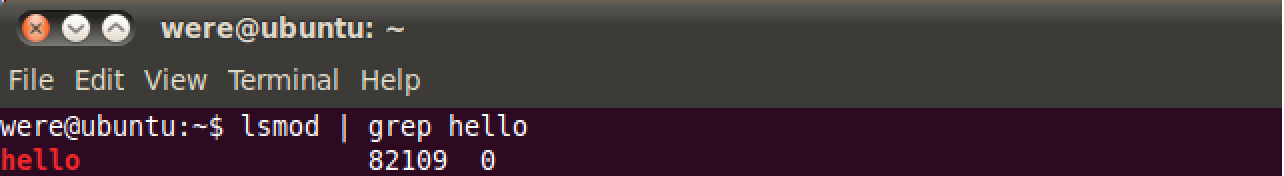
\includegraphics[scale=0.3]{image/not-hidden-ko}
\par\end{centering}

\caption{通过 lsmod 查看当前加载的所有 LKM 模块\label{fig:=00901A=008FC7-lsmod-=0067E5=00770B=005F53=00524D=0052A0=008F7D=007684=006240=006709}}
\end{figure}


但是如果我们在内核中加入隐藏自身的代码, 就能够将其从文件系统和 lsmod 中隐藏起来, 如图 \ref{fig:=0052A0=005165=004EE3=007801=009690=0085CF=00529F=0080FD=00540E,-=004ECE-lsmod}
所示.

\begin{figure}[H]
\begin{centering}
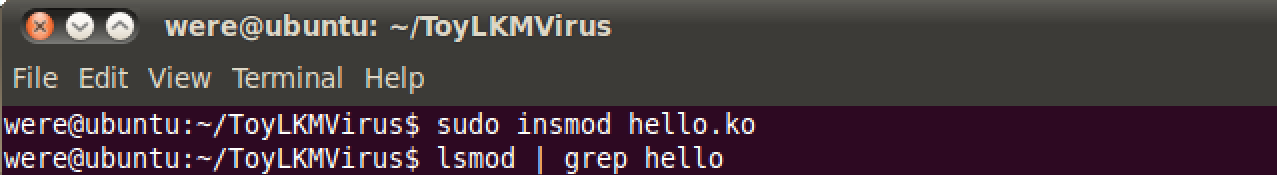
\includegraphics[scale=0.3]{image/hidden-ko}
\par\end{centering}

\caption{加入代码隐藏功能后, 从 lsmod 中隐藏了自身\label{fig:=0052A0=005165=004EE3=007801=009690=0085CF=00529F=0080FD=00540E,-=004ECE-lsmod}}
\end{figure}


TODO: 缺少从 /proc 中隐藏的截图


\section{系统调用劫持}

TODO: 在 find\_syscall\_table 里面用 printk 打印出 syscall\_table 的地址, 用
dmesg 查看. 然后在 \texttt{/boot/System.map{*} }里面 grep 出 syscall\_table
的地址. 两个值应该一致.


\section{病毒的发作}

TODO: mkdir 之后打印 dmesg


\section{进程隐藏}

前面提到, 这个模块具有隐藏进程的功能. 在这个例子中, 它会将指定的以 gedit 开头的进程隐藏起来. 如图 \ref{fig:=009690=0085CF=004EE5-gedit-=005F00=005934=007684=008FDB=007A0B}
所示.

\begin{figure}[H]
\begin{centering}
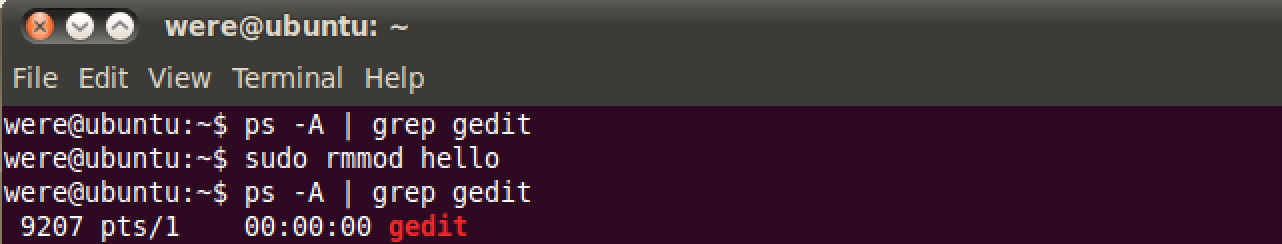
\includegraphics[scale=0.3]{image/hidden-ps}
\par\end{centering}

\caption{隐藏以 gedit 开头的进程\label{fig:=009690=0085CF=004EE5-gedit-=005F00=005934=007684=008FDB=007A0B}}
\end{figure}



\section{病毒的传播}

TODO: 加图
\end{document}
